\addtocontents{toc}{\protect\phasecrisp{Phase 1 --- Compréhension du métier}}
\chapter{Contexte général du projet}

\section*{Introduction}
\addcontentsline{toc}{section}{Introduction}

Ce premier chapitre situe le projet et fixe ce qu'il doit accomplir. Il présente l'organisme d'accueil, étudie
le fonctionnement du support informatique avant notre intervention, en déduit la problématique et
expose la solution retenue. Il traduit ensuite le besoin en exigences vérifiables, puis décrit la
démarche de conduite adoptée.

Une précision de méthode s'impose d'emblée, car elle vaut pour tout le chapitre. Les éléments
relatifs au groupe et à la filiale proviennent de deux sources nommément citées : la présentation
remise lors de la session d'intégration~\cite{otbs-integration} et le site institutionnel de
l'entreprise~\cite{otbs-site}. Tout ce qui concerne le service support et son fonctionnement est
déduit du fichier d'export des tickets, dont le chapitre~3 détaille la constitution. Lorsqu'une
information nous a manqué, nous le disons plutôt que de la combler.

Dans la démarche CRISP-DM, que sa dernière section expose, ce chapitre porte la phase de
compréhension du métier.

\section{Présentation de l'organisme d'accueil}

Le projet s'est déroulé dans une filiale d'un groupe industriel tunisien, au sein d'une
direction restreinte, et sous des règles de confidentialité qui ont pesé sur les choix
techniques dès le premier jour.

\subsection{Le groupe OneTech et sa filiale Business Solutions}

OneTech Group est un groupe industriel tunisien présent sur les marchés de l'automobile, de
l'énergie et de l'industrie. Il revendique quarante années d'expertise sur trois métiers, le câble,
la mécatronique et les technologies de l'information et de la communication, portés par des filiales
spécialisées.

Le groupe déclare un chiffre d'affaires de 325 millions d'euros au titre de l'exercice 2023, une
présence dans plus de cinquante pays et plus de 4\,500 collaborateurs~\cite{otbs-integration}. Ces
trois ordres de grandeur situent l'échelle de l'ensemble auquel appartient notre structure
d'accueil, et expliquent la diversité des filiales que le service support dessert.

\otbs, désignée par le sigle \OTBS dans la suite du mémoire, est la filiale qui porte l'activité des
technologies de l'information. Elle se présente comme un intégrateur indépendant de solutions à
forte valeur ajoutée, du conseil jusqu'à l'exploitation. Son identité visuelle est celle que porte
la figure~\ref{fig:logo-otbs}.

% Logo institutionnel, repris de la page de garde (tpl/cover_page.tex, img/logoSociete.png).
% Place avec [H] plutot que flottant : il doit rester sous le paragraphe de presentation.
\begin{figure}[H]
\centering

\includegraphics[width=0.45\textwidth]{logoSociete.png}
\caption{Logo de \otbs}
\label{fig:logo-otbs}
\end{figure}


Le tableau~\ref{tab:otbs} rassemble les éléments d'identité de l'entreprise, tels que la
présentation d'intégration les énonce.

\begin{table}[!htbp]
\centering
\styletableau
\caption{Éléments d'identité de \OTBS}
\label{tab:otbs}
\begin{tabular}{|Bp{4.6cm}|Lp{9.4cm}|}
\hline
\rowcolor{enteteTab}
\textbf{Élément} & \textbf{Valeur déclarée} \\
\hline
Effectif & 150 collaborateurs \\
\hline
Clients & Plus de 300 \\
\hline
Projets & Plus de 100 par an \\
\hline
Chiffre d'affaires & 37 millions de dinars, soit environ 11 millions d'euros \\
\hline
Ancienneté et implantation & Quarante ans, Afrique et Europe \\
\hline
Siège & 16, rue des Entrepreneurs, Z.I. Charguia II, 2035 Tunis \\
\hline
\end{tabular}
\end{table}

L'activité se répartit sur cinq lignes de métier : les réseaux, les communications et la
collaboration, la sécurité et la conformité, les centres de données et les systèmes, enfin la
gestion et l'exploitation informatique. Sur chacune, l'entreprise intervient depuis l'audit et la
conception jusqu'au déploiement, à la formation et à l'ingénierie logicielle.

Sa clientèle se répartit entre les télécommunications, le pétrole et le gaz, le secteur public et le
secteur financier. Ces domaines partagent une sensibilité marquée à la circulation de leurs données,
ce qui pèse directement sur les choix techniques que nous exposons plus loin.

\subsection{Organisation interne et cadre de confidentialité}

\label{sec:organigramme1}

Six directions se rattachent à la direction générale : les opérations, les systèmes d'information,
la transformation digitale et la communication, les ressources humaines, la direction financière et
la direction Software Solutions.

La figure~\ref{fig:organigramme1} reproduit le document remis par le service, restreint aux cinq
dernières. La branche des opérations, qui réunit à elle seule les directions des projets, des achats
et de la logistique, technique et commerciale, occupe l'autre moitié du document ; la faire tenir
sur la même page ramènerait les libellés sous le seuil de lisibilité, et ce sont les cinq autres qui
situent le projet.

La \textbf{direction des systèmes d'information} héberge ce travail. Placée sous l'autorité de
M. Maher Daassi, elle réunit deux consultants en systèmes d'information, dont notre encadrante
Mme Rahma Oueslati, et une responsable qualité. C'est une équipe de trois personnes, ce qui explique
qu'un projet de cette ampleur y ait été confié à un stagiaire.

Une seconde unité compte pour la suite sans figurer ici. La \textbf{direction technique}, rattachée
aux opérations, porte les compétences que le support mobilise : quatre équipes conduites chacune par
un responsable, Système avec six consultants, Sécurité avec dix dont le responsable de la sécurité
des systèmes d'information, R\&S avec neuf, Voix avec six, complétées d'une coordination BackOffice
et d'une coordination Support. Le découpage de ces quatre équipes recoupe le référentiel de huit
catégories selon lequel le service classe ses tickets.

Une réserve doit être posée sur ce rapprochement. Le service support traite les demandes internes de
l'entreprise et des filiales du groupe, tandis que les équipes de la direction technique
interviennent aussi en prestation chez les clients. L'organigramme dit qui existe et sous quelle
autorité ; il ne dit pas qui prend en charge tel ticket un jour donné. Seul l'export de l'outil de
suivi répond à cette question, et la section~\ref{sec:perimetre1} s'y emploie.

\textbf{Le cadre de confidentialité.} La session d'intégration consacre une section entière aux règles de qualité et de sécurité :
confidentialité des informations, sauvegarde, bureau propre, encadrement de l'accès sans fil,
supervision et vigilance~\cite{otbs-integration}. Ces règles s'appliquent à tout intervenant, stagiaire
compris.

Nous en avons tiré une contrainte de conception, posée avant toute étude technique et jamais
remise en cause depuis : aucune donnée de ticket ne peut être transmise à un service d'intelligence
artificielle hébergé par un tiers. Ce chapitre la formalise en exigence non fonctionnelle, et les
chapitres~4 et~5 montrent ce qu'elle a coûté, en performance comme en temps de réponse.

% Figure placee en fin de sous-section : tout le commentaire, y compris le cadre
% de confidentialite qui clot le propos, se lit d'abord ; l'organigramme referme
% la sous-section. [H] l'empeche de deriver ailleurs.
\begin{figure}[H]
\centering
\includegraphics[width=\textwidth]{ch01_organigramme.pdf}
\caption[Organigramme de \OTBS]{Organigramme de \OTBS, directions rattachées à la direction
générale hors branche des opérations}
\label{fig:organigramme1}
\end{figure}

\section{Cadre du projet}

Cette section étudie le service tel qu'il fonctionnait avant notre intervention, confronte ce
diagnostic aux outils du marché, puis formule la question à laquelle le travail répond. Tout ce qui
suit est déduit du fichier d'export des tickets, dont le chapitre~3 détaille la constitution.

\subsection{Étude de l'existant}

\label{sec:ticketing1}

\textbf{Le ticketing, socle organisationnel du support.} Un système de gestion de tickets
centralise les demandes, les trace et les affecte. Chaque demande y devient un ticket portant une
description, une catégorie, une priorité, un statut et l'historique de son traitement. En disposer
ne garantit pourtant pas un traitement efficace : quand le volume augmente, les consultants restent
absorbés par la lecture des descriptions, la qualification, l'orientation et la recherche d'une
solution déjà appliquée. Ce sont ces opérations que la littérature sur l'automatisation des tickets
cherche à alléger~\cite{alhawari2019,zangari2023}, en qualifiant automatiquement la demande et en
retrouvant les cas semblables, la décision restant au consultant. C'est le principe retenu pour
HelpDesk AI, et les pages qui suivent le confrontent à la situation observée chez \OTBS.

\label{sec:perimetre1}

\textbf{Périmètre et acteurs du service.} Le projet s'est déroulé au sein du service assurant le support informatique interne, sous
l'encadrement de Mme Rahma Oueslati, consultante en systèmes d'information.

L'organigramme de la section~\ref{sec:organigramme1} situe les directions de l'entreprise sans
délimiter ce service : aucune unité ne porte ce nom, la coordination du support y tient en une
personne, et les compétences mobilisées se répartissent entre plusieurs équipes techniques. Nous en
avons donc établi le périmètre à partir des traces qu'il laisse dans son propre outil de suivi, ce
qui décrit l'organisation telle
qu'elle fonctionne et non telle qu'elle est censée fonctionner. Le fichier d'export porte trois
enseignements directs, lisibles par simple dénombrement de valeurs distinctes.

Onze personnes apparaissent comme affectataires de tickets. Notre encadrante figure parmi elles, ce
qui confirme qu'elle traite les demandes en même temps qu'elle encadre. Deux cent deux personnes
apparaissent comme demandeuses. Huit filiales du groupe sont représentées, et la
figure~\ref{fig:entites1} donne leurs volumes respectifs.

\begin{figure}[!htbp]
\centering
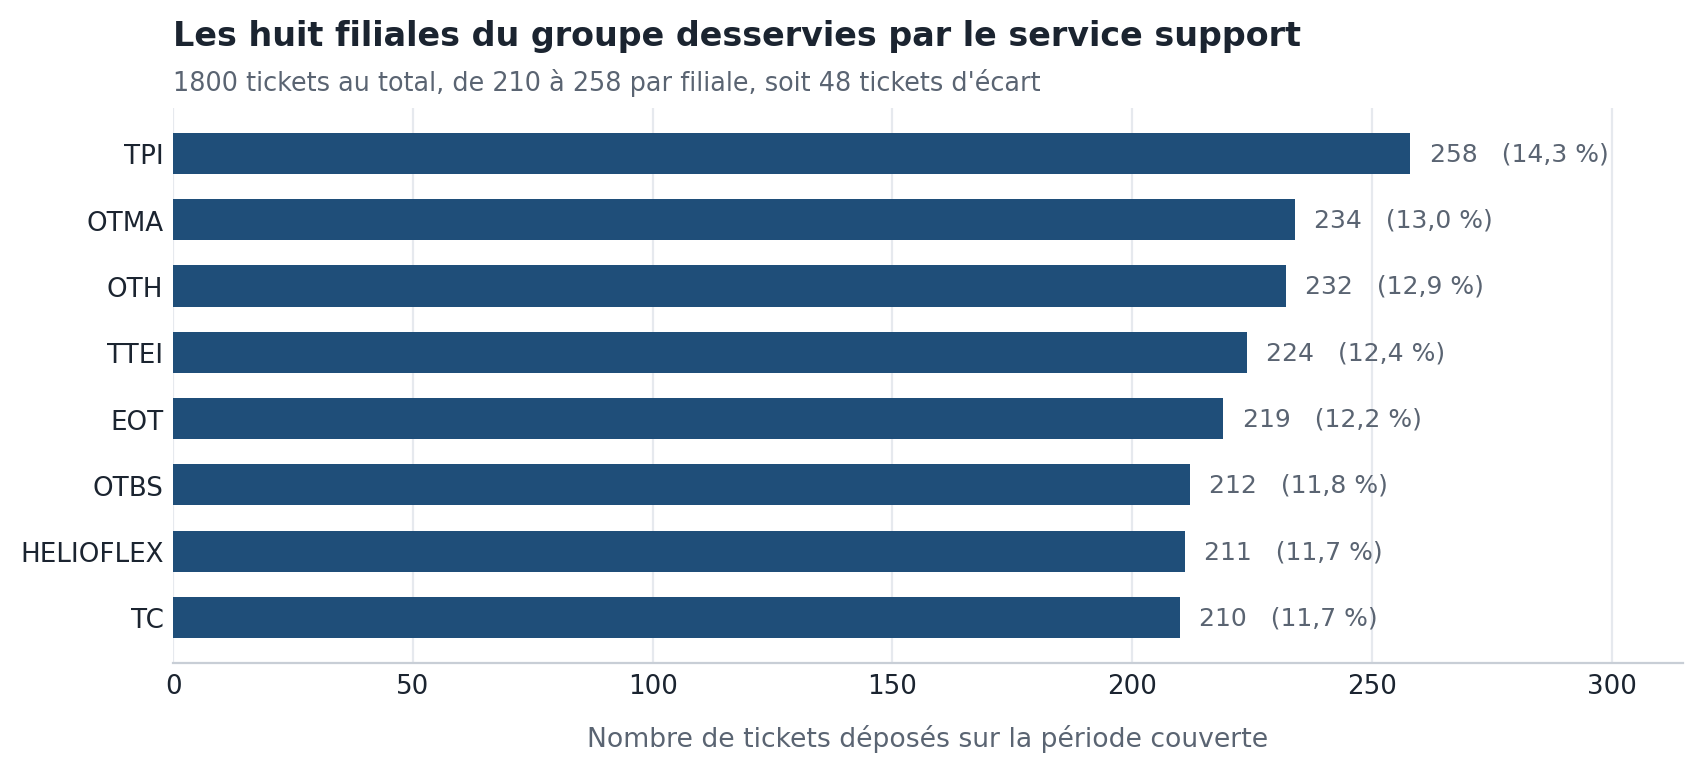
\includegraphics[width=\textwidth]{ch01_repartition_entites.png}
\caption{Répartition des tickets entre les huit filiales desservies}
\label{fig:entites1}
\end{figure}

La charge est remarquablement plate : 48 tickets séparent la filiale la plus demandeuse de la moins
demandeuse, soit un écart de 23\,\% sur des volumes compris entre 210 et 258. Aucune filiale ne
domine le service. Les libellés portés sur la figure sont les codes du fichier d'export, et \OTBS y
figure au même titre que les autres, le service assurant aussi le support de sa propre société.

Le support est donc une fonction mutualisée, servie par une équipe restreinte au profit d'une
population plus de dix-huit fois plus nombreuse. Les applications, les usages et le vocabulaire
varient d'une filiale à l'autre, ce qui élargit la diversité des formulations qu'un modèle de
classification devra absorber.

Les demandes sont classées selon un référentiel de huit catégories : Microsoft, Réseau, Applicatifs,
Infrastructure, Système, Communication, Sécurité et Backup. Leur fréquence est très inégale, le
rapport entre la plus courante et la plus rare atteignant 5,93. Ce déséquilibre constituera la
principale difficulté du travail de modélisation conduit au chapitre~4.

Deux autres classements coexistent avec celui-là dans le fichier. Une colonne de classification
range chaque ticket parmi cinq natures, la demande, le problème, l'incident, l'alerte et le
changement. Une colonne de priorité en distingue quatre, du mineur au critique. Le service dispose
donc déjà d'un vocabulaire de gestion de services, sans qu'aucun de ces trois axes ne soit exploité
autrement que par lecture humaine.

\textbf{Volumétrie observée.} Le corpus couvre quatorze mois, du 1\textsuperscript{er} janvier 2025 au 17 février 2026, pour
1\,800 tickets déposés. La figure~\ref{fig:volumetrie} en donne la répartition mensuelle.

\begin{figure}[!htbp]
\centering
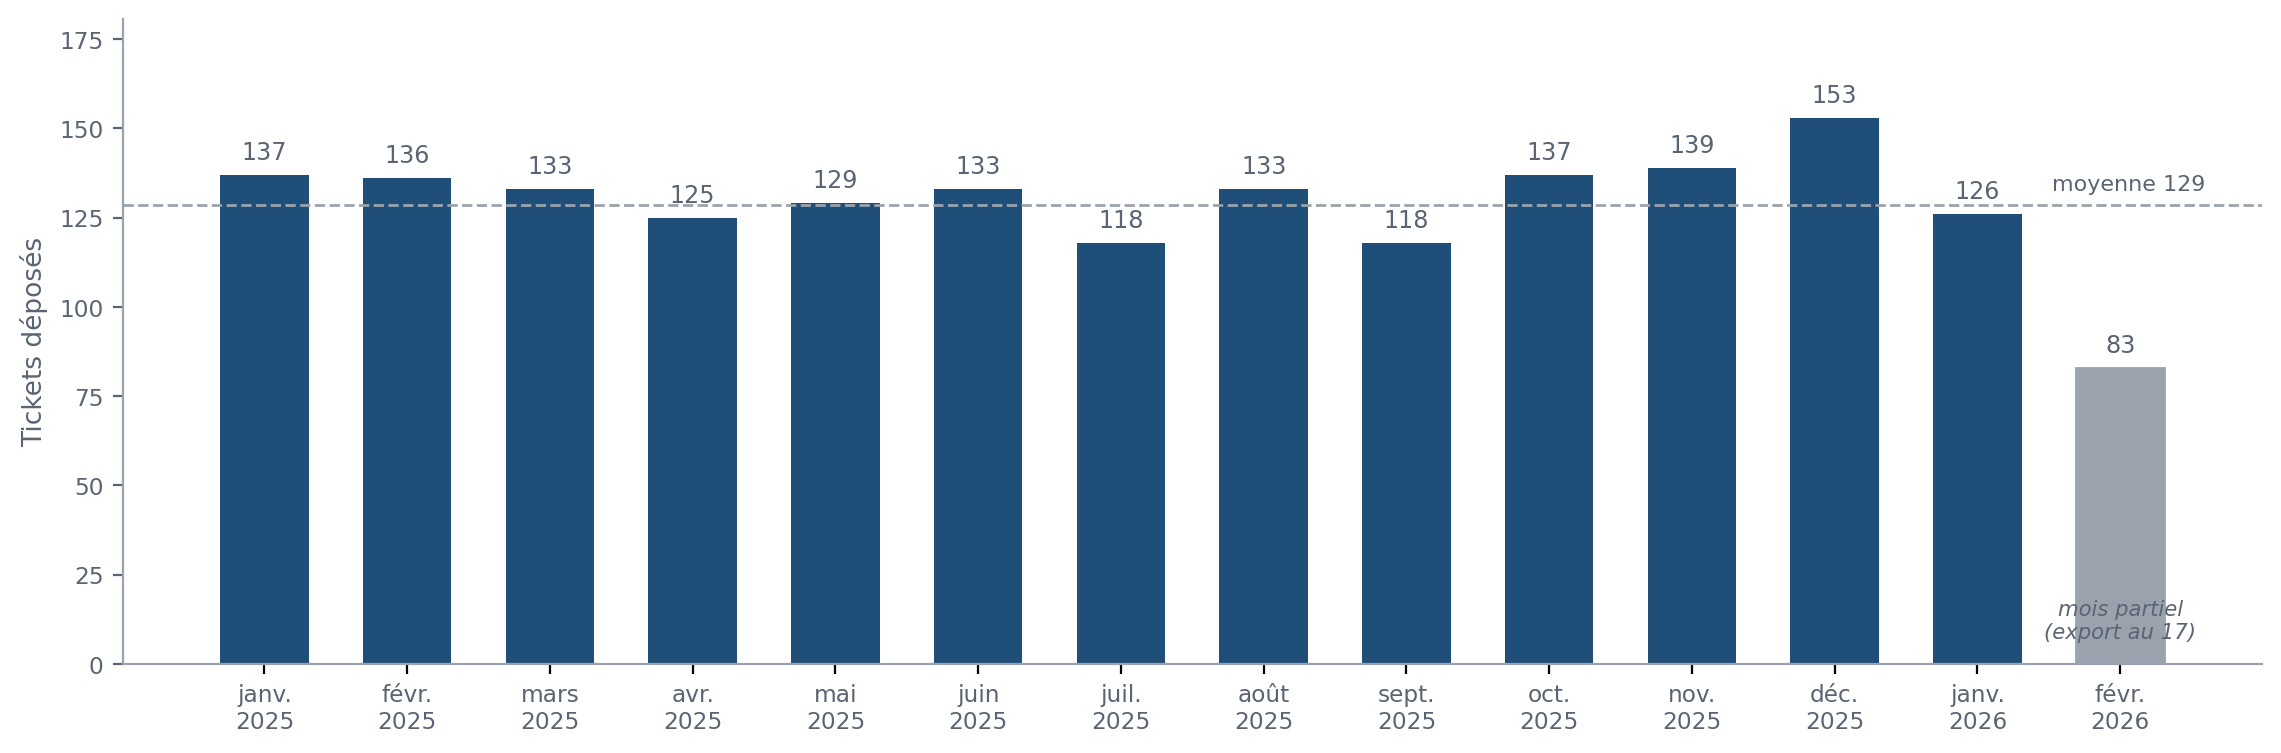
\includegraphics[width=\textwidth]{ch01_volumetrie_mensuelle.png}
\caption{Tickets déposés par mois sur la période couverte par l'export}
\label{fig:volumetrie}
\end{figure}

L'activité est remarquablement stable, autour de 129 tickets par mois, soit environ six par jour
ouvré. Aucune saisonnalité marquée n'apparaît. Le dernier mois est partiel, l'export s'arrêtant au
17 février, et la figure le signale pour éviter d'y lire une chute d'activité.

Cette stabilité a une conséquence pratique pour la suite. Un service dont la charge ne varie pas
n'a pas de pic à absorber, et le gain attendu d'une assistance automatique ne réside donc pas dans
l'écrêtage d'une surcharge. Il réside dans le temps passé, ticket après ticket, sur des gestes que
la section~\ref{sec:repetitivite} montre concentrés sur un petit nombre de cas.

\textbf{L'outil de suivi et la qualité de ses données.} L'enregistrement reposait sur une liste SharePoint. Nous ne le déduisons pas d'un entretien mais du
fichier d'export : la colonne \texttt{Chemin d'accès} porte, sur les 1\,800 lignes et sans exception,
la valeur \texttt{sites/IT-Check/Lists/HelpDesk}. Une telle liste assure la saisie et
l'historisation, sans offrir ni tri automatique ni recherche dans les résolutions passées. Surtout,
elle ne contient que ce qu'un consultant a pris le temps d'y consigner.

L'export porte dix-huit colonnes, dont six ne sont pas systématiquement renseignées : la
priorité, l'affectation, l'analyse, la résolution, l'identifiant de rattachement et la date de
résolution. Le chapitre~2 en donne les taux et les interprète, la qualité des données relevant de
l'étude du corpus plutôt que de l'état des lieux du service.


Un défaut plus discret mérite d'être signalé, car il illustre ce qu'une saisie sans contrôle
produit. La colonne des dates de création mêle deux formats, 972 lignes au format jour, mois, année
et 828 au format année, mois, jour. Une lecture naïve du fichier n'en interprète qu'un seul et perd
silencieusement 46\,\% du corpus. Le chapitre~3 revient sur les nettoyages que cet état de fait a
rendus nécessaires.

\textbf{Le cycle de vie du ticket.} Le processus n'ayant jamais été formalisé, nous l'avons déduit des données. Le champ \texttt{STATUT}
prend cinq valeurs qui décrivent un cycle de vie complet, restitué à la figure~\ref{fig:processus}.

\begin{figure}[!htbp]
\centering
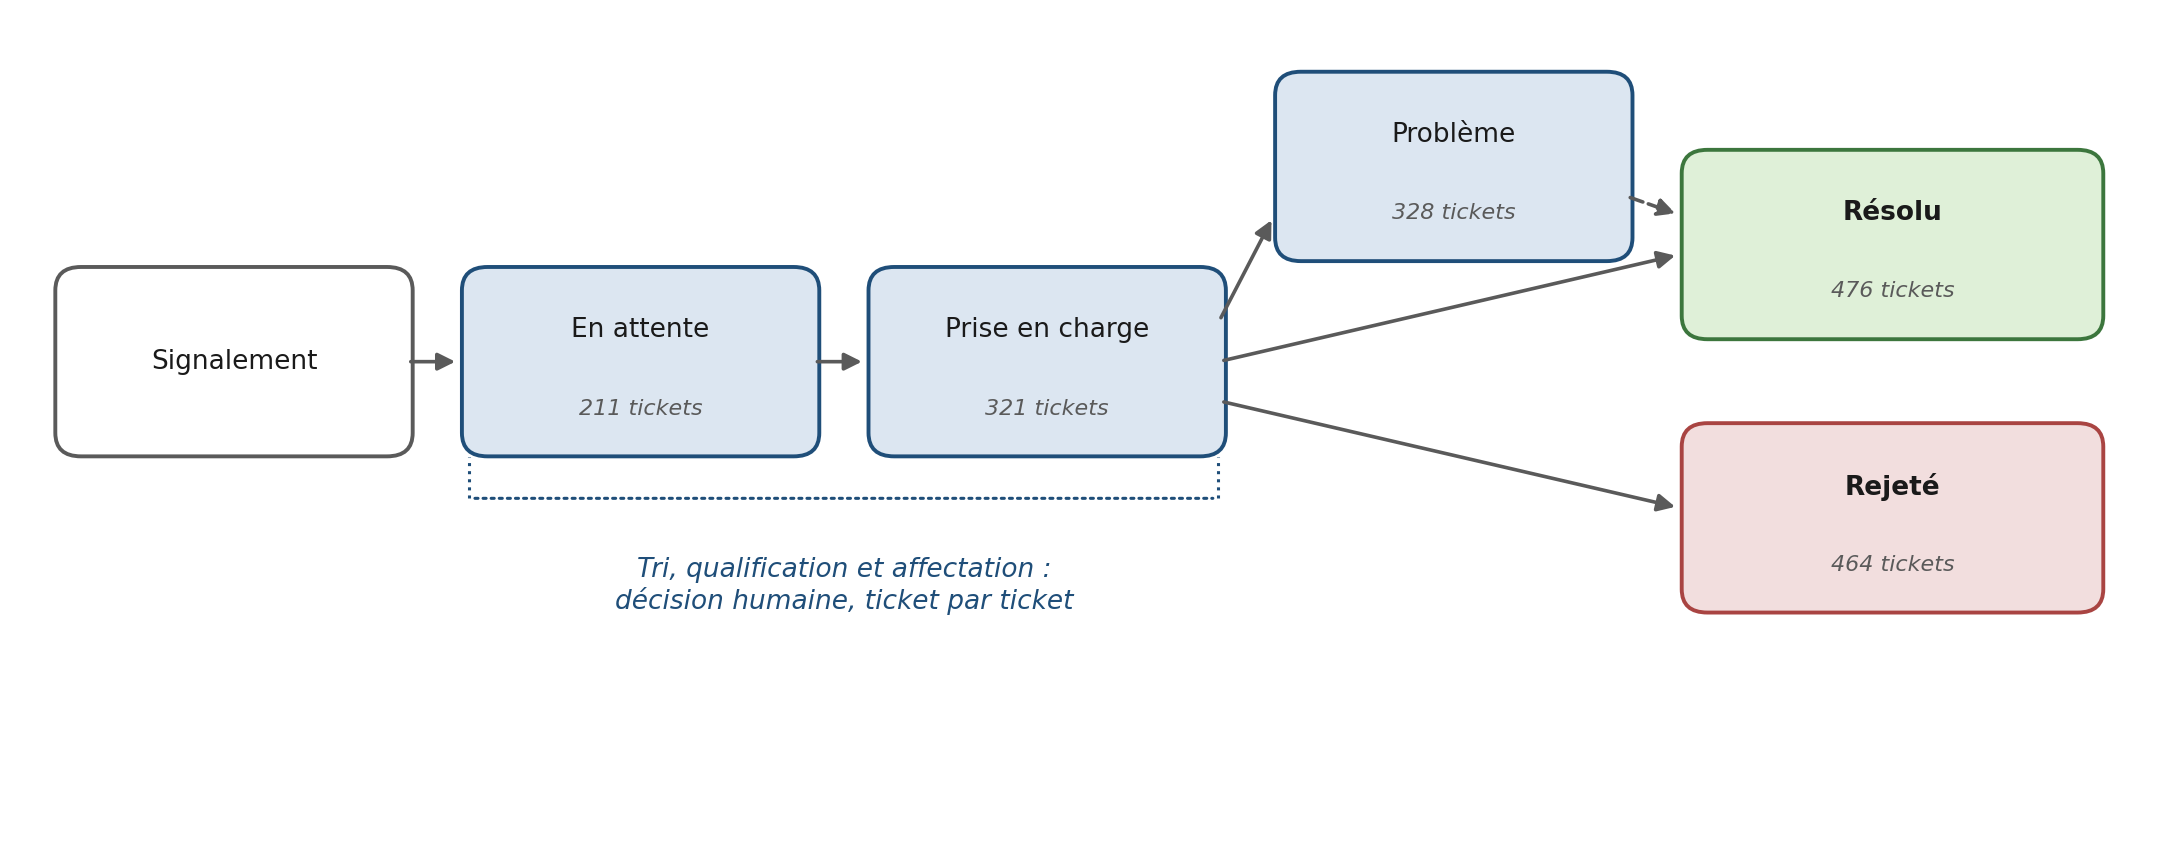
\includegraphics[width=\textwidth]{ch01_processus_existant.png}
\caption{Cycle de vie du ticket avant le projet, reconstitué à partir du champ \texttt{STATUT}}
\label{fig:processus}
\end{figure}

Le tri, la qualification et l'affectation se logent entre le dépôt et la prise en charge. Ce sont
des décisions humaines, prises ticket après ticket, et le fichier n'en garde aucune trace autre que
leur résultat. L'étape de qualification commande tout le reste, car décider de la catégorie d'un
ticket revient à décider qui va le traiter. Une catégorie mal choisie oriente la demande vers une
compétence qui n'est pas la bonne, et le temps est perdu deux fois. La classification automatique
que nous proposons répond d'abord à ce besoin d'aiguillage.

Un chiffre retient l'attention sur cette figure : 464 tickets rejetés pour 476 résolus. Près d'une
demande sur deux parvenue à son terme se solde par un refus. Ce taux renseigne moins sur la
difficulté des cas soumis au service que sur l'absence de contrôle à l'entrée. Le fichier
n'enregistre aucun motif structuré de rejet, et nous ne pouvons donc pas en décomposer les causes.

\label{sec:repetitivite}

\textbf{Répétitivité des résolutions.} Une dernière observation achève de caractériser ce travail. Sur les 1\,800 tickets du corpus, la
colonne consacrée aux gestes de résolution ne compte que 58 valeurs distinctes. Les colonnes de
titre, d'analyse et de base de connaissances en comptent exactement autant, ce qui indique qu'elles
sont solidaires : le service traite cinquante-huit situations types, répétées une trentaine de fois
chacune en moyenne.

Les descriptions libres, elles, comptent 1\,535 valeurs distinctes. L'écart entre ces deux nombres
résume le problème du service. Les utilisateurs formulent leurs demandes de mille manières, alors
que les réponses appartiennent à un répertoire restreint et stable. Retrouver la bonne réponse est
un travail de reconnaissance, non d'invention.

Le temps des consultants se concentre alors sur des tâches sans valeur ajoutée technique :
qualifier la demande pour l'orienter, retrouver un cas comparable dans l'historique, rédiger la
réponse au demandeur. Aucune n'exige l'expertise pour laquelle ils ont été recrutés.

\textbf{Limites du diagnostic.} L'honnêteté du diagnostic exige d'en marquer les bords. Plusieurs éléments qu'un état des lieux
complet comporterait nous ont manqué, faute de réponse à la demande d'informations adressée à
l'entreprise. Nous les énonçons ici plutôt que de les combler par des suppositions.

Nous ne disposons ni d'organigramme du service, ni de description de ses niveaux d'intervention, ni
d'engagement de niveau de service formalisé. Le fichier ne dit rien du canal par lequel chaque
demande est arrivée, de sorte que la part des sollicitations passées par téléphone ou de vive voix
reste inconnue. Le temps moyen de traitement d'un ticket n'a pas été confirmé, et nous ne le citons
donc nulle part dans ce mémoire. Enfin, le motif des rejets n'est pas structuré dans les données.

Ces manques limitent la portée du diagnostic sur un point précis : nous ne pouvons pas chiffrer le
gain de temps attendu de la plateforme. Ils ne l'affaiblissent pas sur ce que les données montrent
directement, à savoir la répétitivité du travail, le déséquilibre des catégories, le taux de rejet
et l'absence de mémoire interrogeable. Ce risque est suivi au registre du projet.

\subsection{Limites de l'existant et solutions du marché}

Le tableau~\ref{tab:limites} met les limites constatées en regard du besoin qu'elles engendrent.

\begin{table}[!htbp]
\centering
\styletableau
\caption{Limites de l'existant et besoins associés}
\label{tab:limites}
\begin{tabular}{|Bp{6.6cm}|Lp{7.4cm}|}
\hline
\rowcolor{enteteTab}
\textbf{Limite constatée} & \textbf{Besoin qui en découle} \\
\hline
Aucun point d'entrée ne garantit qu'une intervention laisse une trace &
Offrir un point d'entrée unique et structuré \\
\hline
Le demandeur n'a aucune visibilité sur l'avancement de sa demande &
Donner au demandeur un suivi autonome de ses tickets \\
\hline
L'orientation du ticket repose sur un jugement manuel, refait à chaque demande &
Proposer automatiquement une catégorie, assortie d'un indicateur de fiabilité \\
\hline
L'historique des résolutions n'est pas interrogeable &
Retrouver les cas comparables et leurs sources à partir d'une description libre \\
\hline
La connaissance produite reste attachée aux personnes &
Capitaliser automatiquement chaque résolution validée \\
\hline
La saisie n'est soumise à aucun contrôle, d'où des champs vides et des formats mêlés &
Contrôler la saisie à la source plutôt qu'après coup \\
\hline
\end{tabular}
\end{table}

Ces limites partagent une même origine : le dispositif en place enregistre une partie de
l'information, après coup, sans jamais l'exploiter.

\textbf{Les solutions du marché.} Trois familles d'outils auraient pu répondre au besoin, et aucune ne le fait entièrement dans notre
contexte.

Les plateformes en mode service, telles Zendesk ou Freshdesk, supposent l'hébergement des données
chez l'éditeur, ce que la contrainte de confidentialité exclut d'emblée. Les solutions libres
hébergeables en interne, GLPI au premier rang, assurent la gestion du cycle de vie du ticket sans
proposer nativement de classification apprise sur l'historique du service. Les suites complètes de
gestion des services informatiques, du type ServiceNow, sont dimensionnées pour des organisations
d'une tout autre échelle que celle d'une équipe de onze personnes.

Le tableau~\ref{tab:marche1} confronte ces trois familles aux trois exigences que le contexte
impose. Aucune colonne n'est pleine, et c'est ce constat qui fonde la problématique du projet.

\begin{table}[!htbp]
\centering
\singlespacing
\styletableau
\renewcommand{\arraystretch}{1.25}
\caption{Les trois familles d'outils du marché face aux exigences du contexte}
\label{tab:marche1}
\begin{tabular}{|Lp{4.0cm}|Cp{3.1cm}|Cp{3.1cm}|Cp{3.3cm}|}
\hline
\rowcolor{enteteTab}
\textbf{Exigence du contexte} &
\textbf{Plateformes en mode service}\newline \small\textit{Zendesk, Freshdesk} &
\textbf{Solutions libres hébergeables}\newline \small\textit{GLPI} &
\textbf{Suites complètes de gestion}\newline \small\textit{ServiceNow} \\
\hline
Les données ne quittent pas l'infrastructure de l'entreprise &
\cellcolor{refus}\textbf{Non}\newline \small hébergement chez l'éditeur &
\cellcolor{tenu}\textbf{Oui} &
\cellcolor{tenu}\textbf{Oui} \\
\hline
Classification apprise sur l'historique propre au service &
\cellcolor{tenu}\textbf{Oui} &
\cellcolor{refus}\textbf{Non}\newline \small pas de classification native &
\cellcolor{tenu}\textbf{Oui} \\
\hline
Dimensionnement adapté à une équipe de onze personnes &
\cellcolor{tenu}\textbf{Oui} &
\cellcolor{tenu}\textbf{Oui} &
\cellcolor{refus}\textbf{Non}\newline \small échelle bien supérieure \\
\hline
\end{tabular}
\end{table}

Aucune famille ne réunit simultanément le traitement du français métier tel que ce service l'écrit,
l'exécution sur l'infrastructure de l'entreprise et l'exploitation de l'historique propre au
service.

\subsection{Problématique}

\begin{center}
\begin{minipage}{0.92\textwidth}
\itshape
Comment classer automatiquement et de manière fiable des tickets informatiques francophones, courts,
déséquilibrés et bruités, et proposer une assistance à la résolution pertinente et vérifiable, tout
en conservant un contrôle humain sur la décision finale ?
\end{minipage}
\end{center}

\vspace{2mm}

Cette problématique se décline en questions de recherche qui structurent les travaux des
chapitres~4 et~5. Un modèle de langue francophone spécialisé améliore-t-il significativement la
classification par rapport à une approche lexicale classique, en particulier sur les catégories
minoritaires ? Une recherche sémantique fondée sur des représentations vectorielles denses
surpasse-t-elle une recherche lexicale ? Comment calibrer la confiance du modèle pour définir un
seuil au-delà duquel sa proposition peut être tenue pour suffisamment sûre ?

\section{Solution proposée et périmètre du travail}

Nous proposons une plateforme, nommée HelpDesk AI, dont la figure~\ref{fig:solution} donne la vue
fonctionnelle.

\begin{figure}[!htbp]
\centering
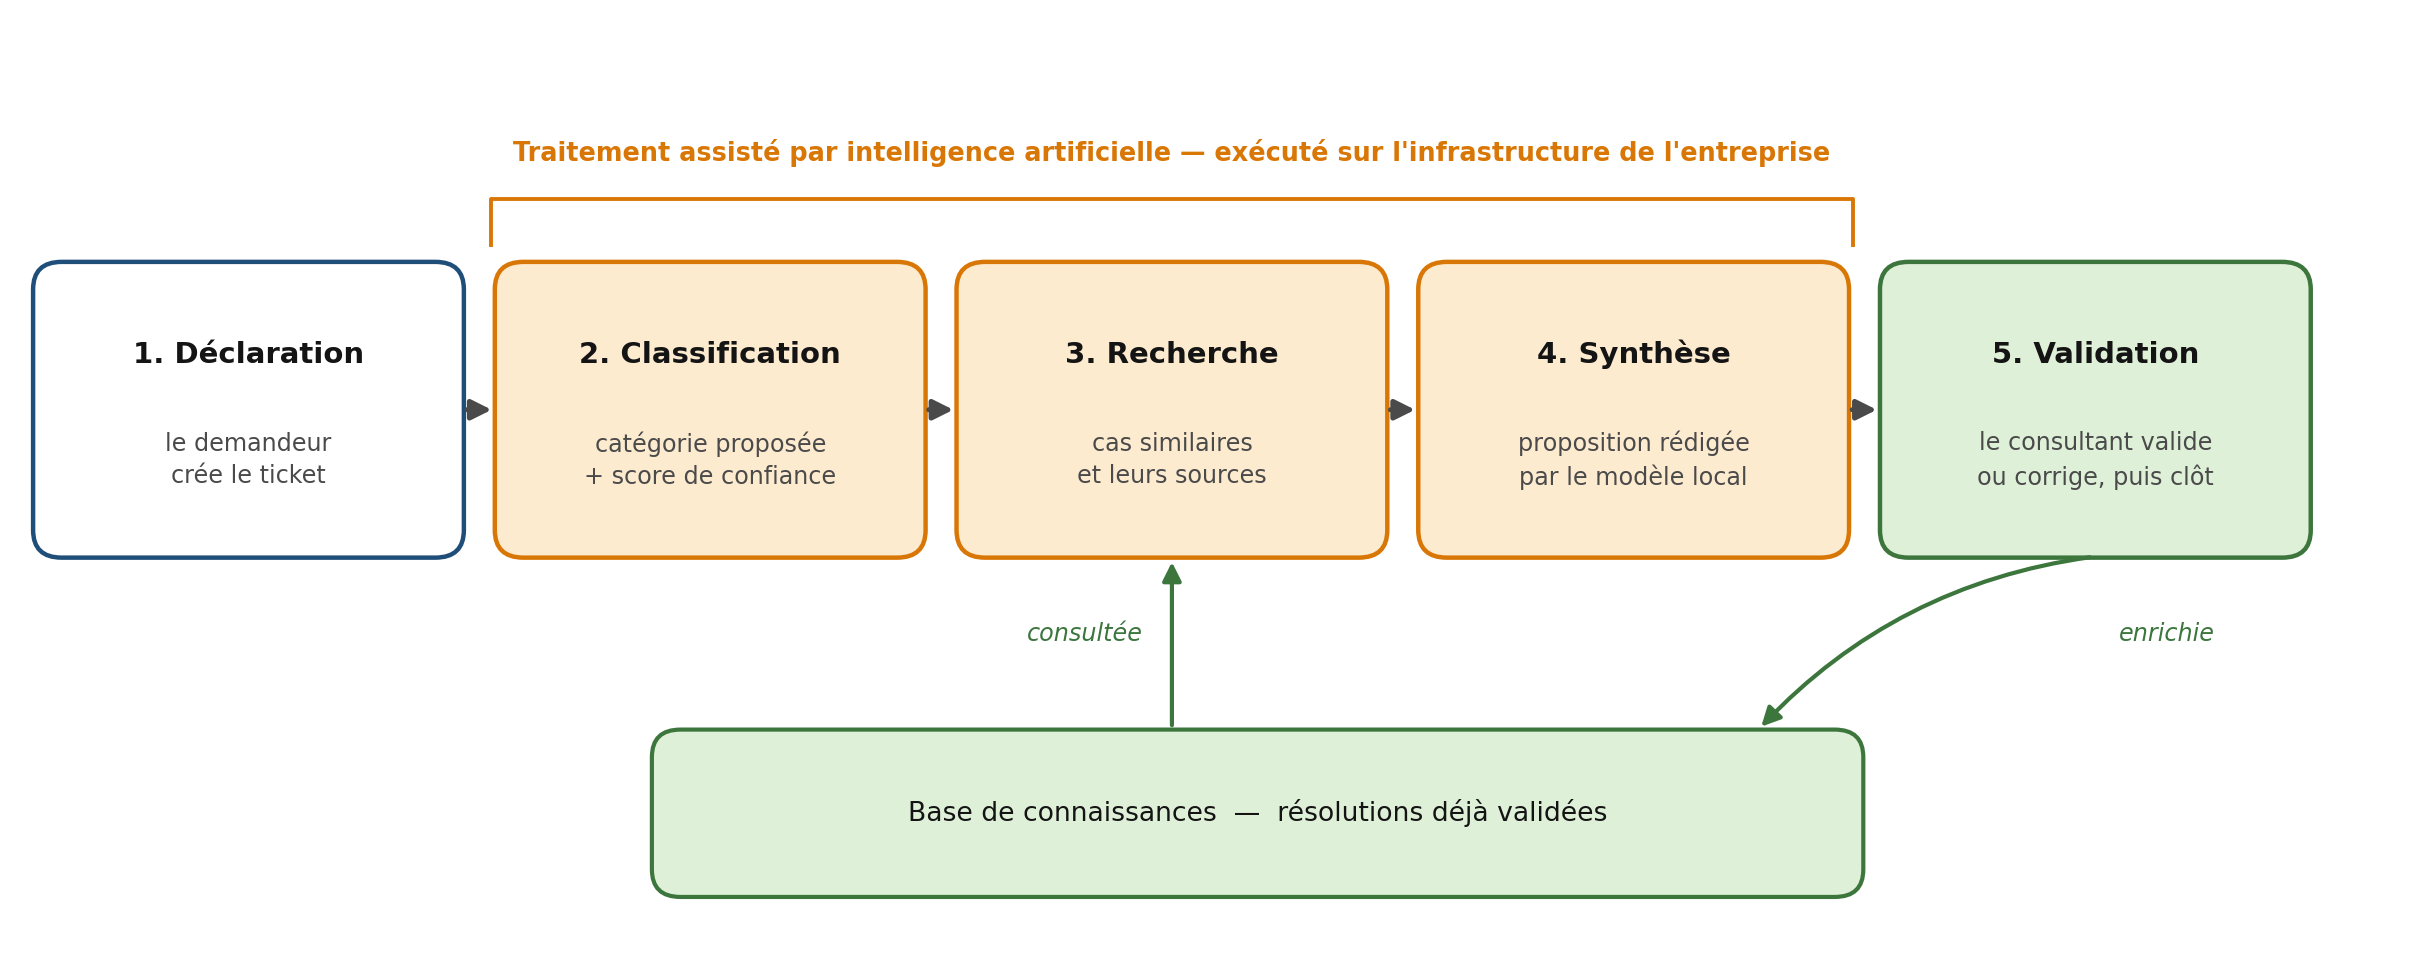
\includegraphics[width=\textwidth]{ch01_vue_solution.png}
\caption{Vue fonctionnelle de la solution proposée}
\label{fig:solution}
\end{figure}

Elle est d'abord le point d'entrée qui faisait défaut : toute demande y est déclarée par le
demandeur lui-même dans un formulaire structuré, de sorte qu'aucune intervention n'échappe plus à
l'historique. Viennent ensuite les briques d'assistance. Le classifieur automatique attribue une
catégorie à chaque ticket entrant et retourne un score de confiance, qui appuie la décision
d'orientation. Le moteur de recherche par similarité interroge l'historique des résolutions et
remonte les cas les plus proches avec leurs sources, de sorte que chaque suggestion reste
vérifiable. Le modèle de langage exécuté localement synthétise enfin ces cas en une proposition
rédigée, sans qu'aucune donnée ne quitte l'infrastructure de l'entreprise.

Le principe directeur est le maintien de la décision humaine : le système propose, le consultant
tranche. Aucune décision n'est appliquée sans validation, et chaque validation alimente en retour la
base de connaissances. L'application distingue en conséquence deux parcours, un portail où le
demandeur crée et suit ses tickets, et une console d'administration où le consultant examine les
propositions, les corrige si nécessaire et clôt les demandes.

\textbf{Périmètre du travail.} Reste à délimiter le périmètre, ce que fait le tableau~\ref{tab:perimetre}. Poser cette frontière
dès le cadrage protège l'évaluation contre le reproche de ne pas avoir traité ce qui n'a jamais été
promis.

\begin{table}[!htbp]
\centering
\styletableau
\caption{Périmètre retenu et hors-périmètre}
\label{tab:perimetre}
\begin{tabular}{|Bp{6.9cm}|Lp{7.1cm}|}
\hline
\rowcolor{enteteTab}
\textbf{Inclus dans le périmètre} & \textbf{Exclu du périmètre} \\
\hline
Chaîne de données documentée, versionnée et reproductible &
Mise en production sur l'infrastructure du groupe \\
\hline
Classifieur automatique évalué sur protocole explicite &
Intégration au système d'information existant \\
\hline
Moteur d'assistance à la résolution et modèle de langage local &
Reprise et migration des tickets historiques \\
\hline
Application web complète, portail demandeur et console d'administration &
Notifications automatiques sur changement de statut \\
\hline
Conteneurisation et chaîne de traitement reproductible &
Supervision en exploitation et reprise sur incident \\
\hline
\end{tabular}
\end{table}

Le livrable attendu est une plateforme démontrable et documentée, accompagnée d'une évaluation
honnête de ce qu'elle apporte et de ses limites. Sa mise en exploitation reste hors sujet.

\textbf{Les contraintes qui ont pesé.} Quatre contraintes ont pesé sur le travail du cadrage jusqu'à la
soutenance. Le
tableau~\ref{tab:contraintes1} les réunit avec ce que chacune a écarté.

\begin{table}[!htbp]
\centering
\singlespacing
\styletableau
\renewcommand{\arraystretch}{1.15}
\caption{Contraintes du projet, leur origine et ce qu'elles ont écarté}
\label{tab:contraintes1}
\begin{tabular}{|Bp{2.9cm}|Lp{5.4cm}|Lp{4.8cm}|}
\hline
\rowcolor{enteteTab}
\textbf{Contrainte} & \textbf{Origine} & \textbf{Ce qu'elle a écarté} \\
\hline
Confidentialité des tickets &
Règles de sécurité de l'entreprise, énoncées à la session d'intégration et reprises en ENF-04 &
Les services d'inférence hébergés. Le modèle de langage s'exécute sur place, ce qui pèse sur le
temps de réponse \\
\hline
Un corpus étroit &
L'historique que le service a pu fournir : 1\,800 lignes, 58 types de demandes, 8 catégories dont
deux réunissent moins de cinq pour cent des tickets &
L'entraînement d'un modèle depuis zéro. Le travail porte sur l'adaptation d'un modèle déjà
pré-entraîné \\
\hline
Un matériel modeste &
Le processeur graphique mis à disposition dispose de 2\,Go de mémoire vidéo &
L'ajustement complet d'un transformer. L'adaptation à faible rang répond à cette limite \\
\hline
La décision reste humaine &
Principe posé au cadrage avec le service support &
La clôture prononcée par le système. Toute demande passe par une file d'approbation \\
\hline
\end{tabular}
\end{table}

Ces contraintes ne sont pas des obstacles rencontrés en chemin. Elles étaient connues au cadrage,
elles commandent les choix techniques des chapitres~4 et~5, et le chapitre~6 chiffre ce qu'elles ont
coûté.

\label{sec:positionnement2}

\textbf{Ce que le travail apporte en propre.} Les techniques mobilisées sont d'usage courant. Ce
qui distingue ce travail tient aux conditions dans lesquelles elles sont mises en œuvre et à ce que
nous avons choisi de mesurer : l'apport de règles métier ajoutées à un modèle statistique, mesuré au
lieu d'être supposé, et des scores obtenus sous un découpage qui regroupe les tickets par type avant
le tirage, précaution qui empêche un même type de demande de figurer à la fois dans l'apprentissage
et dans l'évaluation. Les chapitres~4 et~6 rapportent ces mesures. Elles valent dans les limites de
leur cadre : un seul service, une seule entreprise, un corpus francophone dont la faible diversité
interdit de présumer que les résultats se transporteraient ailleurs.

\section{Analyse et spécification des besoins}

\label{sec:besoins1}

Le besoin décrit plus haut se traduit ici en exigences vérifiables, chacune portant un
identifiant auquel les chapitres suivants se réfèrent.

\subsection{Objectifs du projet}
\label{sec:objectifs1}

Sept objectifs résument ce que la plateforme doit accomplir. Doter le service d'un point
d'entrée unique où aucune demande n'échappe à l'historique. Proposer une catégorie à chaque
demande entrante, sans laisser passer celles qui relèvent de la sécurité. Remonter des
résolutions passées comparables avec leurs sources, et les présenter assez vite pour que l'outil
soit préféré à la lecture directe du ticket. Laisser la décision à l'administrateur, aucune
clôture n'étant prononcée par le système. Rendre enfin la chaîne de traitement des données et
des modèles rejouable à l'identique.

Chacun se traduit dans les pages qui suivent en exigences numérotées, dont le critère
d'acceptation permet au chapitre~6 de conclure sans avoir à juger du résultat.

\subsection{Acteurs du système}

La plateforme distingue deux profils, récapitulés au tableau~\ref{tab:acteurs}. Cette distinction se
traduit directement dans le contrôle d'accès RBAC de l'application, qui ne connaît que deux rôles.

\begin{table}[!htbp]
\centering
\styletableau
\caption{Acteurs du système et responsabilités associées}
\label{tab:acteurs}
\begin{tabular}{|Bp{3.4cm}|Cp{2.2cm}|Lp{8.2cm}|}
\hline
\rowcolor{enteteTab}
\textbf{Acteur} & \textbf{Rôle} & \textbf{Responsabilités} \\
\hline
Demandeur & \texttt{client} & Créer une demande, suivre son avancement, consulter la réponse
apportée \\
\hline
Administrateur & \texttt{admin} & Traiter les tickets : consulter la qualification proposée et les
cas comparables avec leurs sources, valider ou corriger, répondre au demandeur. Superviser
l'activité : volumes, catégories, délais, gestion des comptes \\
\hline
\end{tabular}
\end{table}

Les administrateurs sont les consultants du service support eux-mêmes ; le terme désigne leur rôle
dans l'application, non une fonction distincte dans l'organisation. Ce regroupement du traitement et
de la supervision s'écarte des référentiels de gestion de services informatiques, qui séparent
l'agent du responsable. Cette séparation n'aurait ici aucun objet : le service compte onze
consultants qui traitent les demandes et suivent collectivement l'activité, sans échelon
intermédiaire.

Le demandeur n'a délibérément aucune visibilité sur les mécanismes de classification : ni la
catégorie prédite ni l'index de confiance ne lui sont présentés. Exposer une prédiction incertaine à
un utilisateur non spécialiste reviendrait à lui faire porter un arbitrage qui ne lui revient pas.

\subsection{Besoins fonctionnels}

Chaque exigence porte un critère d'acceptation vérifiable et un niveau de priorité : \textbf{élevée}
lorsqu'elle conditionne la livraison, \textbf{moyenne} lorsque son report resterait acceptable,
\textbf{faible} pour un apport de confort. Le tableau~\ref{tab:ef} les regroupe par niveau ; la
colonne \emph{Domaine} rappelle à quelle partie du parcours du ticket chacune se rattache.

\begin{table}[!htbp]
\centering
\styletableau
\caption{Exigences fonctionnelles et critères d'acceptation}
\label{tab:ef}
% Meme interligne resserre que le tableau des exigences non fonctionnelles :
% les deux tableaux de specification gardent ainsi la meme densite.
\renewcommand{\arraystretch}{1.25}
\begin{tabular}{|Cp{1.3cm}|Lp{4.2cm}|Lp{5.1cm}|Lp{2.5cm}|}
\hline
\rowcolor{enteteTab}
\textbf{Réf.} & \textbf{Exigence} & \textbf{Critère d'acceptation} & \textbf{Domaine} \\
\hline
\multicolumn{4}{|l|}{\cellcolor{enteteTab}\textbf{Priorité élevée} : conditionne la livraison} \\
\hline
EF-01 & Authentification et gestion des rôles & Accès restreint selon le rôle, jeton vérifié à chaque appel & Cycle de vie \\
\hline
EF-02 & Création d'un ticket par le demandeur & Ticket persisté, statut initial renseigné & Cycle de vie \\
\hline
EF-03 & Journal d'audit des modifications & Chaque changement tracé avec son auteur et sa date & Cycle de vie \\
\hline
EF-04 & Suivi du ticket par le demandeur & Statut et réponse consultables & Cycle de vie \\
\hline
EF-05 & Classification automatique en catégorie & Catégorie et index de confiance retournés & Traitement \\
\hline
EF-06 & Recherche de cas comparables & Trois résolutions proposées avec leurs sources & Traitement \\
\hline
EF-07 & Orientation selon l'index de confiance & Cas peu assurés dirigés vers une revue humaine & Traitement \\
\hline
EF-08 & Validation ou correction par l'administrateur & Catégorie finale et solution enregistrées & Qualité \\
\hline
\multicolumn{4}{|l|}{\cellcolor{enteteTab}\textbf{Priorité moyenne} : le report resterait acceptable} \\
\hline
EF-09 & Synthèse rédigée à l'attention du consultant & Réponse formulée, sources citées, garde-fous actifs & Traitement \\
\hline
EF-10 & Recueil du retour du demandeur & Avis persisté et exploitable & Qualité \\
\hline
EF-11 & Résumé automatique du ticket & Résumé affiché à l'administrateur & Qualité \\
\hline
EF-12 & Suggestion de priorité & Niveau proposé à la prise en charge & Qualité \\
\hline
\multicolumn{4}{|l|}{\cellcolor{enteteTab}\textbf{Priorité faible} : apport de confort} \\
\hline
EF-13 & Analyse de tonalité du message & Indicateur d'urgence affiché & Qualité \\
\hline
EF-14 & Tableau de bord d'activité & Volumes, catégories et délais consultables & Qualité \\
\hline
\end{tabular}
\end{table}

% Le commentaire qui suit porte sur le tableau : la barriere empeche le flottant
% de deriver apres lui, ce qui ferait lire l'explication avant la piece expliquee.

Le classement en trois niveaux suit les dépendances du parcours d'un ticket. Les huit exigences de
priorité élevée forment la chaîne minimale sans laquelle une demande ne peut ni exister, ni être
qualifiée, ni être tranchée : la déposer (EF-02), la qualifier (EF-05, EF-06, EF-07), décider de son
sort (EF-08), la suivre (EF-04) et savoir qui est intervenu (EF-01, EF-03). En retirer une seule
interrompt le parcours décrit plus haut, et la solution cesse alors de répondre au problème qui
l'a motivée.

Les exigences de priorité moyenne allègent le travail du consultant sans conditionner ce parcours.
Un ticket se traite sans synthèse rédigée ni résumé automatique : le consultant lit la description
lui-même, comme il le faisait avant l'outil. Celles de priorité faible n'interviennent pas dans le
traitement d'une demande ; elles servent à observer l'activité une fois celle-ci traitée.

Une exigence appelle une réserve, posée ici plutôt que laissée à la découverte du lecteur :
l'exigence EF-09 s'appuie sur des gabarits de texte et non sur une génération libre par le modèle
de langage.

\subsection{Besoins non fonctionnels}

Les exigences non fonctionnelles fixent les seuils que la solution devra tenir, et ce sont eux que le chapitre~6 confrontera aux mesures.

% Placement [H] : le tableau doit suivre immediatement le titre de la sous-section.
% En [!htbp] il flottait vers la page suivante et laissait une demi-page blanche.
\begin{table}[H]
\centering
\styletableau
\caption{Exigences non fonctionnelles}
\label{tab:enf}
% Interligne resserre et colonne d'exigence elargie : neuf lignes tiennent ainsi
% sous le titre de la sous-section, au lieu d'imposer une page a elles seules.
\renewcommand{\arraystretch}{1.05}
\begin{tabular}{|Cp{1.4cm}|Bp{3.2cm}|Lp{9.4cm}|}
\hline
\rowcolor{enteteTab}
\textbf{Réf.} & \textbf{Catégorie} & \textbf{Exigence} \\
\hline
ENF-01 & Performance & Prédiction et recherche servies sous 300\,ms au quatre-vingt-quinzième centile \\
\hline
ENF-02 & Qualité de l'IA & F1-macro du classifieur d'au moins 0,85, mesuré selon un protocole arrêté
avant l'expérimentation \\
\hline
ENF-03 & Qualité de l'IA & Rappel d'au moins 0,70 sur la catégorie \emph{Sécurité} \\
\hline
ENF-04 & Confidentialité & (a) Aucune donnée de ticket transmise à un service externe ;
(b) traitement des données personnelles conforme à la réglementation \\
\hline
ENF-05 & Sécurité & Authentification par jeton, contrôle d'accès RBAC, secrets non exposés \\
\hline
ENF-06 & Fiabilité & Fonctionnement dégradé mais opérationnel en cas d'indisponibilité du modèle de
langage \\
\hline
ENF-07 & Maintenabilité & Code structuré en couches et couvert par des tests automatisés \\
\hline
ENF-08 & Reproductibilité & Chaîne de traitement des données et des modèles réexécutable à l'identique \\
\hline
ENF-09 & Portabilité & Déploiement conteneurisé sur une infrastructure standard \\
\hline
\end{tabular}
\end{table}

Le tableau~\ref{tab:enf} référence les exigences non fonctionnelles sur le même principe que les
exigences fonctionnelles, de sorte que les chapitres suivants puissent s'y référer sans ambiguïté.

Ces neuf exigences ne proviennent pas d'un référentiel appliqué par principe. Chacune répond à une
propriété que le service attendait ou à une contrainte qui s'imposait au projet. Le temps de réponse
(ENF-01) tient à ce qu'un outil plus lent que la lecture directe d'un ticket ne serait pas adopté.
Le rappel sur la catégorie \emph{Sécurité} (ENF-03) tient à ce qu'elle compte parmi les plus rares du
référentiel et que l'erreur y coûte le plus cher. Le fonctionnement dégradé (ENF-06) tient à ce que
le modèle de langage s'exécute sur une machine de l'entreprise, donc peut cesser de répondre.

L'exigence ENF-04 occupe une place à part. Les autres se négocient, une latence pouvant être améliorée ou
une couverture de tests complétée. Celle-ci traduit une règle interne de l'entreprise et une
obligation réglementaire sur les données personnelles. Elle a été traitée comme un axiome de
conception, et c'est elle qui a imposé l'exécution locale du modèle de langage.

Ses deux volets n'ont cependant pas connu le même sort, et nous les distinguons dès leur énoncé
pour que le bilan du chapitre~6 puisse les juger séparément. Le volet (a), l'absence de service
externe, relève de l'architecture et se vérifie dans le code livré. Le volet (b), le traitement des
données personnelles, se partage entre un traitement technique et une décision d'organisation :
pseudonymisation du corpus d'un côté, durée de conservation et information des personnes de
l'autre. Le premier a été mis en œuvre et vérifié ; les deux autres dépassent le cadre du stage, et
présenter le volet comme entièrement satisfait serait inexact. La section~\ref{sec:rgpd} en
détaille la portée exacte, et le bilan du chapitre~6 le déclare partiellement tenu.

\textbf{Traçabilité des exigences.} Le tableau~\ref{tab:tracabilite} rattache chaque domaine d'exigences au chapitre qui en rend compte.
La conclusion générale revient sur celles que la solution livrée ne tient pas.

\begin{table}[!htbp]
\centering
\styletableau
\caption{Traçabilité des exigences vers les chapitres de traitement}
\label{tab:tracabilite}
\begin{tabular}{|Bp{6.4cm}|Cp{2.2cm}|Lp{4.6cm}|}
\hline
\rowcolor{enteteTab}
\textbf{Domaine d'exigences} & \textbf{Chapitre} & \textbf{Nature du traitement} \\
\hline
Gouvernance et qualité des données & 3 & Constitution du corpus, séparation anti-fuite,
versionnement \\
\hline
Classification automatique, qualité de l'IA & 4 & Comparaison des approches, évaluation \\
\hline
Assistance à la résolution, confidentialité & 5 & Moteur de similarité, modèle de langage local \\
\hline
Cycle de vie, accès, boucle de qualité & 7 & Application web, workflow, validation humaine \\
\hline
Sécurité, fiabilité, reproductibilité, portabilité & 3 et 7 & Traitement transverse au fil des
chapitres, bilan de conformité au chapitre~6 \\
\hline
\end{tabular}
\end{table}

\section{Méthodologie de travail}

Le projet mêle du développement logiciel, dont le résultat se planifie, et de
l'expérimentation, dont le résultat ne se planifie pas. Le choix d'une démarche devait
tenir compte des deux.

\subsection{Comparaison des démarches envisagées}

Trois démarches de conduite ont été examinées avant de trancher, chacune portant une
conception différente de ce qui peut être planifié à l'avance.

\begin{table}[H]
\centering
% Place avec [H] pour rester sous le titre. Le paquet float court-circuite le
% reglage d'interligne que setspace applique aux flottants : on le retablit ici.
\singlespacing
\styletableau
\caption{Comparaison des démarches de conduite de projet}
\label{tab:methodo}
\begin{tabular}{|Bp{3.1cm}|Lp{3.5cm}|Lp{3.5cm}|Lp{3.5cm}|}
\hline
\rowcolor{enteteTab}
\textbf{Critère} & \textbf{Cycle en V} & \textbf{Scrum} & \textbf{CRISP-DM} \\
\hline
Nature du besoin & Figé en amont & Évolutif & Exploratoire \\
\hline
Progression & Séquentielle, une seule passe & Itérative, incréments livrables & Itérative, retours
entre phases \\
\hline
Gestion de l'incertitude & Faible & Bonne sur le produit & Bonne sur la donnée \\
\hline
Livrable intermédiaire & Documents de spécification & Incrément fonctionnel & Modèle évalué \\
\hline
Limite dans notre contexte & Les résultats d'un modèle ne se planifient pas & Ne couvre pas le cycle
de vie de la donnée & Ne décrit pas le développement applicatif, rattaché ici au déploiement \\
\hline
\end{tabular}
\end{table}

Le tableau~\ref{tab:methodo} compare sur cinq critères les trois démarches examinées.
Le projet relève de deux natures de travail que les démarches classiques traitent rarement ensemble.
Il comporte un volet de développement logiciel, où le besoin est identifiable et le résultat
prévisible, et un volet de science des données, où le résultat d'une expérimentation ne peut par
définition être garanti à l'avance. Nous avons examiné trois démarches candidates.

Le cycle en V suppose un besoin stabilisé et un résultat prévisible ; il aurait conduit à figer des
objectifs de performance avant toute expérimentation, ce qui n'a pas de sens en apprentissage
automatique. Scrum apporte l'itération et la livraison incrémentale, en restant centré sur le
produit logiciel et en laissant de côté la préparation et l'évaluation des données. CRISP-DM
\cite{wirth2000} structure précisément le cycle de vie de la donnée, de la compréhension du métier
jusqu'au déploiement en passant par la préparation, la modélisation et l'évaluation ; il ignore en
revanche le développement applicatif qui doit rendre le modèle utilisable.

\subsection{Démarche retenue : CRISP-DM}

CRISP-DM est la méthodologie officielle de ce projet. C'est le seul des trois cadres examinés qui
traite la préparation et l'évaluation des données comme des étapes à part entière, alors qu'elles
concentrent l'essentiel de la difficulté ici. La figure~\ref{fig:crispdm} en donne la représentation
usuelle.

% Schema fourni par l'auteur (images/crisp.jpg). Il mesure 552x510 px, ce qui donne
% environ 145 dpi a cette largeur : lisible a l'ecran, un peu doux a l'impression.
% Un export du meme schema en 1500 px de large reglerait le point sans rien changer ici.
\begin{figure}[H]
\centering
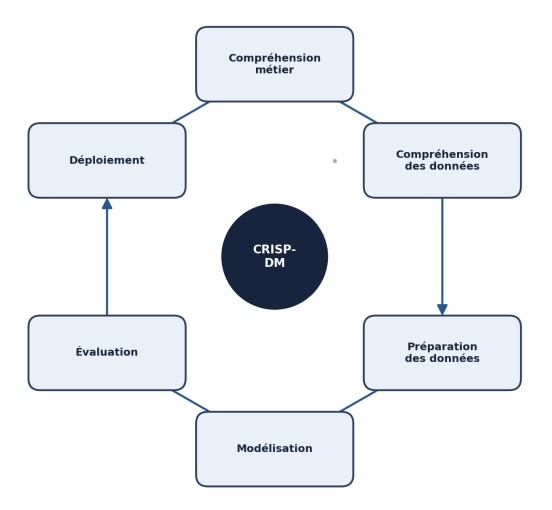
\includegraphics[width=0.62\textwidth]{ch01_crispdm.jpg}
\caption{Les six phases de la démarche CRISP-DM}
\label{fig:crispdm}
\end{figure}

Le schéma se lit comme un cycle fermé : la compréhension du métier l'ouvre, le déploiement y ramène.
C'est ce bouclage qui a joué ici. L'analyse du corpus, au chapitre~2, a fait apparaître une
contrainte que l'entretien initial n'avait pas révélée, et le chapitre~6 rapporte des résultats qui
contredisent l'hypothèse de départ. Chaque retour de ce genre a ouvert une itération nouvelle, où la
question de départ était reposée avant que le travail technique ne reprenne.

Le développement logiciel ne constitue pas une phase supplémentaire. Il se répartit entre la phase
de déploiement et d'intégration, qui dans le standard comprend la production du mécanisme de
livraison, et les itérations successives du projet. L'application du chapitre~7 est ce qui rend les
modèles utilisables, la conteneurisation du chapitre~7 ce qui les rend installables ailleurs.

La figure~\ref{fig:phases1} place les six phases en regard des sept chapitres.

\begin{figure}[H]
\centering
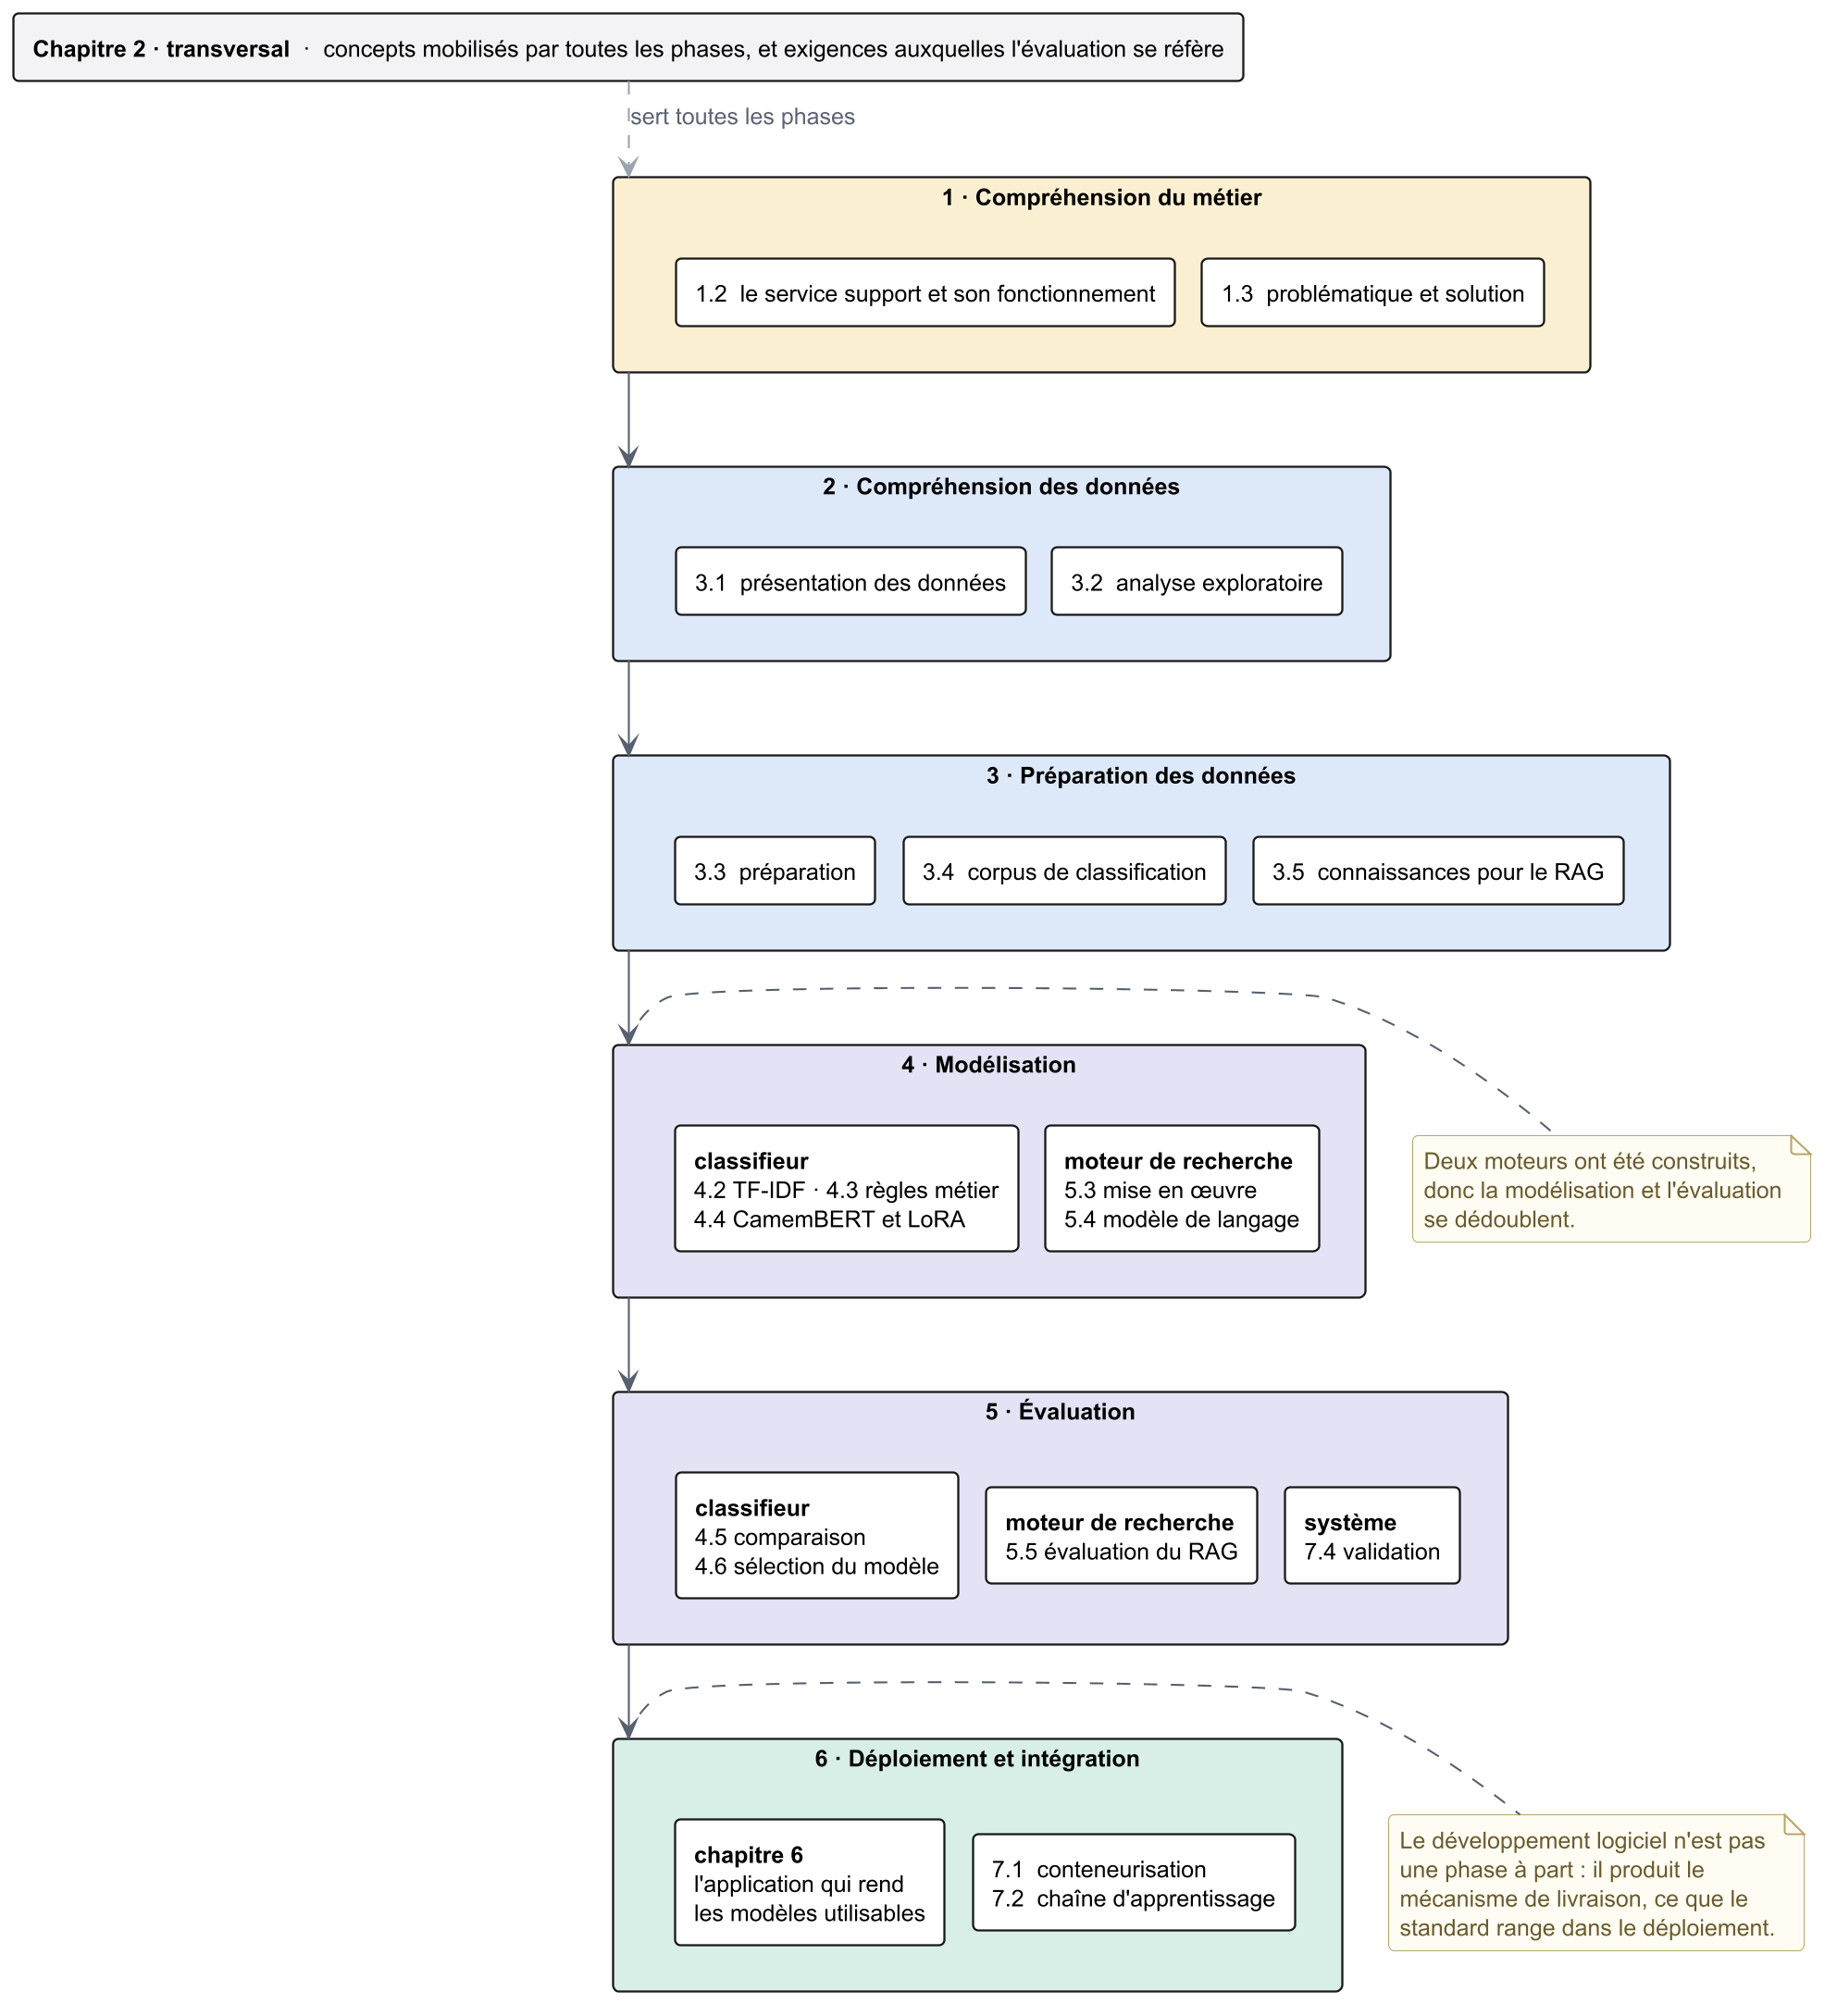
\includegraphics[width=0.98\textwidth]{ch01_crispdm_chapitres.png}
\caption{Les six phases de CRISP-DM en regard des sept chapitres du mémoire}
\label{fig:phases1}
\end{figure}

Deux traits de ce découpage méritent d'être énoncés. La modélisation et l'évaluation se dédoublent,
parce que le travail a produit deux moteurs et non un, chacun avec sa propre campagne de mesure. Et
tout n'est pas rattaché à une phase unique : les concepts théoriques sont exposés dans le chapitre qui les mobilise plutôt que rassemblés à part, et deux sections le sont également, la gouvernance des
données en 3.6 et la chaîne d'apprentissage automatisé en 7.2.

Une règle a été tenue d'un bout à l'autre, et elle engage la validité des résultats : le protocole
d'évaluation de chaque modèle a été arrêté avant son entraînement. Définir la métrique avant
l'expérimentation ferme la porte au biais qui consiste à retenir a posteriori l'indicateur le plus
flatteur. Le chapitre~6 en donne l'illustration, les résultats y étant rapportés tels qu'ils sont
sortis, y compris lorsqu'ils contredisent l'hypothèse initiale.

% Aucun flottant du corps ne doit franchir la conclusion.
\FloatBarrier

\section*{Conclusion}
\addcontentsline{toc}{section}{Conclusion}

Ce chapitre a posé le terrain du projet. Le support informatique d'\OTBS est une fonction
mutualisée : onze consultants traitent les demandes de huit filiales du groupe, pour deux cent deux
demandeurs. Les interventions sont consignées dans une liste SharePoint qui ne trie rien
automatiquement et que personne ne peut interroger.

Trois familles d'outils du marché ont été examinées. Aucune ne réunit à la fois le traitement du
français tel que ce service l'écrit, l'exécution sur l'infrastructure de l'entreprise et
l'exploitation de l'historique propre au service. Nous avons donc conçu une plateforme spécifique,
articulée autour d'un point d'entrée unique, d'un classifieur, d'un moteur de recherche par
similarité et d'un modèle de langage exécuté localement, chaque décision restant soumise à la
validation d'un consultant.

Le besoin est désormais traduit en exigences numérotées, auxquelles le chapitre~6 confrontera les
mesures. La conduite du travail suit CRISP-DM, dont les six phases commandent le découpage des
chapitres qui suivent. Le prochain ouvre la deuxième phase : comprendre les données avant de
prétendre en tirer quoi que ce soit.
